\documentclass[11pt, a4paper, twoside]{article}

% Version en 2024 Víctor Bettachini < vbettachini@unlam.edu.ar >

\usepackage[T1]{fontenc}
\usepackage[utf8]{inputenc}

% \usepackage[spanish, es-tabla]{babel}
% \def\spanishoptions{argentina} % Was macht dass?
% \usepackage{babelbib}
% \selectbiblanguage{spanish}
% \addto\shorthandsspanish{\spanishdeactivate{~<>}}

\usepackage{graphicx}
\graphicspath{{../figuresLaTeX/}}
% \usepackage{float}

\usepackage[arrowdel]{physics}
\newcommand{\pvec}[1]{\vec{#1}\mkern2mu\vphantom{#1}}
% \usepackage{units}
\usepackage[separate-uncertainty= true, multi-part-units= single, range-units= single, range-phrase= {~a~}, locale= FR]{siunitx}
\usepackage{isotope} % $\isotope[A][Z]{X}\to\isotope[A-4][Z-2]{Y}+\isotope[4][2]{\alpha}

\usepackage{tasks}
\usepackage[inline]{enumitem}
% \usepackage{enumerate}

\usepackage{hyperref}

% \usepackage{amsmath}
% \usepackage{amstext}
% \usepackage{amssymb}

\usepackage{tikz}
\usepackage{tikz-3dplot}
\usepackage{tikz-dimline}
\usetikzlibrary{calc}
% \usetikzlibrary{math}
\usetikzlibrary{arrows.meta}
\usetikzlibrary{snakes}
\usetikzlibrary{decorations}
\usetikzlibrary{decorations.pathmorphing}
\usetikzlibrary{patterns}

\usepackage[hmargin=1cm,vmargin=3cm, top= 0.75cm,nohead]{geometry}

\usepackage{lastpage}
\usepackage{fancyhdr}
\pagestyle{fancyplain}
\fancyhf{}
\setlength\headheight{28.7pt} 
\fancyhead[LE, LO]{\textbf{Computational Analytical Mechanics} }
% \fancyhead[LE, LO]{\textbf{Mecánica General} }
\fancyhead[RE, RO]{\href{https://ingenieria.unlam.edu.ar/}{$\vcenter{\hbox{\includegraphics[height=1cm]{ambos.pdf}}}$}}
\fancyfoot{\href{https://creativecommons.org/licenses/by-nc-sa/4.0/}{$\vcenter{\hbox{\includegraphics[height=0.4cm]{by-nc-sa_80x15.pdf}}}$} \href{https://ingenieria.unlam.edu.ar/}{DIIT - UNLaM}}
\fancyfoot[C]{ {\tiny Updated \today} }
\fancyfoot[RO, LE]{Page \thepage/\pageref{LastPage}}
\renewcommand{\headrulewidth}{0pt}
\renewcommand{\footrulewidth}{0pt}



\begin{document}

\begin{center}
  \textsc{\large Generalized coordinates | Constraints | Kinetic and potential energies}
\end{center}
\noindent
Exercises marked with (*) have extra difficulty, don't hesitate to ask for help.

\begin{enumerate}

\item
	\begin{minipage}[t][2.5cm]{0.7\textwidth}
		\textbf{Pendulum with free point of support} [Landau \S5 ex. 2]\\
		Particle of mass $m_2$ is hanging from a rigid bar of length $\ell$ and negligible mass. On the other end there is a device of mass $m_1$ linked to a horizontal bar, and it's free to move horizontally along the $x$ axis. The device allows the hanging bar to span any angle $\varphi$ with respect to the vertical axis. 
	\end{minipage}
	\begin{minipage}[c][2cm][t]{0.3\textwidth}
		\includegraphics[width=0.75\textwidth]{figures/landauS52_fig2.png}
	\end{minipage}
	\begin{enumerate}
		\item After determining the generalized coordinates, write the position of each particle as a function of them.
		\item Calculate the velocity of each particle.
		\item Using these velocities, calculate the kinetic energy, $T$, and potential energy, $V$, for each particle.
		\item Now calculate $T$ and $V$ using the functions with the masses and positions as inputs. Verify that you get the same result but in fewer steps.		
		\item Perform the necessary substitutions into the expressions for $T$ and $V$ found in the previous step, so that the particle with mass $m_1$ remains at rest. Verify that you recover the expressions of $T$ and $V$ of an ideal pendulum.
	\end{enumerate}



\item
	\begin{minipage}[t][3.7cm]{0.7\textwidth}
		\textbf{Double coplanar pendulum} [Landau \S5 ex. 1]\\
		A ridig bar of lentgh $\ell_1$ and negligible mass has a particle of mass $m_1$ attached to one end. There is a second bar of negligible mass hanging from the first one, of length $\ell_2$, with a particle of mass $m_2$ attached to the other end too.		
	\end{minipage}
	\begin{minipage}[c][2cm][t]{0.3\textwidth}
		\includegraphics[width=0.75\textwidth]{figures/landauS52_fig1.png}
	\end{minipage}

	\begin{enumerate}
		\item Write expressions for kinetic energy, $T$, and potential energy, $V$, as functions of the generalized coordinates suggested by the figure.
		
		Result:\\
	\(
		T_\text{translational} = \frac{\ell_{1}^{2} m_{1} \dot{\varphi}_{1}^{2}}{2} + \frac{m_{2} \left(\ell_{1}^{2} \dot{\varphi}_{1}^{2} + 2 \ell_{1} \ell_{2} \cos{\left(\varphi_{1} - \varphi_{2} \right)} \dot{\varphi}_{1} \dot{\varphi}_{2} + \ell_{2}^{2} \dot{\varphi}_{2}^{2}\right)}{2}\\
		V_\text{gravitational} = - g \left(\ell_{1} m_{1} \cos{\left(\varphi_{1} \right)} + \ell_{1} m_{2} \cos{\left(\varphi_{1} \right)} + \ell_{2} m_{2} \cos{\left(\varphi_{2} \right)}\right)
	\)
		\item Use the \verb'subs' function of \verb'SymPy' to set $m_1=0$, $\varphi_1 = \varphi_2 = \varphi$ and  $\ell_1 = \ell_2 = \frac{\ell}{2}$. 
		Verify that you recover the expressions of $T$ and $V$ of an ideal pendulum.
	\end{enumerate}


\item
	\begin{minipage}[t][7.1cm]{0.5\textwidth}
		(*) \textbf{Pendulum with rotating point of support} [Marion (e) ex. 7.5] [Landau \S5 ex. 3]\\
		A particle of mass $m$ is attached to the end of a rigid bar of length $b$. The point of support is linked to a vertical circle of radius $a$ and it rotates with constant frequency $\omega$. It is assumed that all positions lie in the same plane and the mass of the bar is negligible. Calculate the kinetic energy, $T$, and potential $V$, of the particle of mass $m$.

		Result:\\
		\(
			T_\text{translational} = \dfrac{m \left(a^{2} \omega^{2} - 2 a b \omega \sin{\left(\omega t - \theta \right)} \dot{\theta} + b^{2} \dot{\theta}^{2}\right)}{2}\\
			V_\text{gravitational} = g m \left(a \sin{\left(\omega t \right)} - b \cos{\left(\theta \right)}\right)
		\)
	\end{minipage}
	\begin{minipage}[c][3cm][t]{0.5\textwidth}
		\includegraphics[width=0.75\textwidth]{figures/marion_fig7_3.png}
	\end{minipage}



\item
	\begin{minipage}[t][7cm]{0.65\textwidth}
		(*) \textbf{Coupled weights rotating about a vertical axis} [Landau \S5 ex. 4]\\
		Particle with mass $m_2$ moves on a vertical axis and the whole system rotates about this axis with a constant angular velocity $\Omega$. This particle is linked to two particles of mass $m_1$ through bars of length $a$ and negligible mass, and at the same time, these particles are linked to the fixed point $A$ through identical bars, forming the variable angle $\theta$ with respect to the vertical axis.
		Calculate the kinetic energy of each of the three particles and find a compact expression of the kinetic energy of the whole system. Do the same for the potential energy.

		Result:\\
		\(
			T_\text{translational} = a^{2} \left( m_{1} \left( \Omega^{2} \sin^{2}{\left(\theta \right)} + \dot{\theta}^{2}\right) + 2 m_{2} \sin^{2}{\left(\theta \right)} \dot{\theta}^{2} \right) \\
			V_\text{gravitational} = - 2 a g \left(m_{1} + m_{2}\right) \cos{\left(\theta \right)}
		\)
	\end{minipage}
	\begin{minipage}[c][1cm][t]{0.35\textwidth}
		\includegraphics[width=0.75\textwidth]{figures/landauS52_fig4.png}
	\end{minipage}

	\begin{center}
		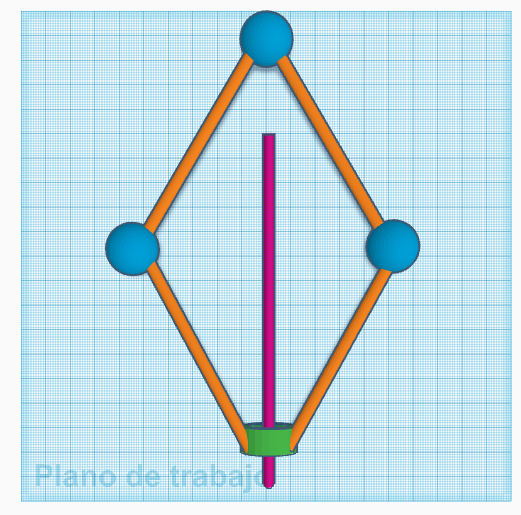
\includegraphics[width=0.35\textwidth]{figures/rotantesAcopladas1.png}
		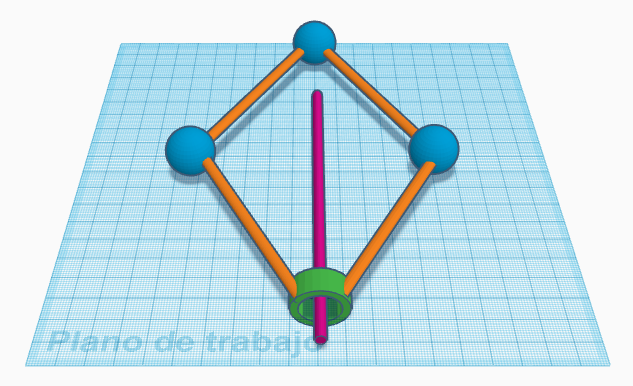
\includegraphics[width=0.35\textwidth]{figures/rotantesAcopladas2.png}
	\end{center}

	In these figures, the top sphere is the fixed point \(A\). Everything revolves around the pink axis with constant angular speed $\Omega$. Therefore, the particles on each side, of mass $m_1$, rotate entering and leaving the plane shown in the first image. This is equivalent to thinking that the lightblue plane rotates around the pink axis.

	The piece of mass $m_2$ is a sliding hub that moves vertically without friction. 
	
	\begin{center}
		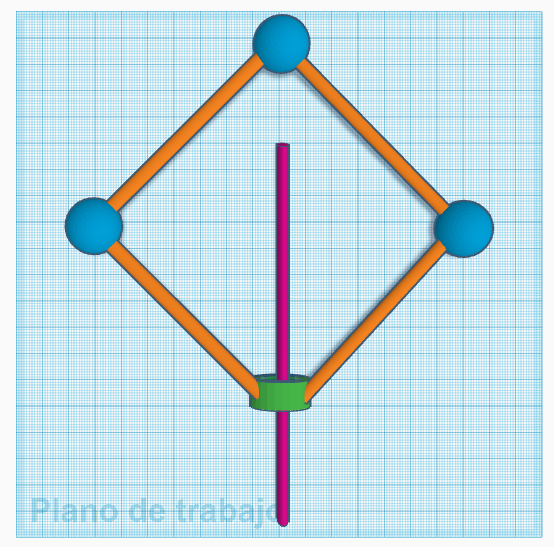
\includegraphics[width=0.35\textwidth]{figures/rotantesAcopladas3.png}
		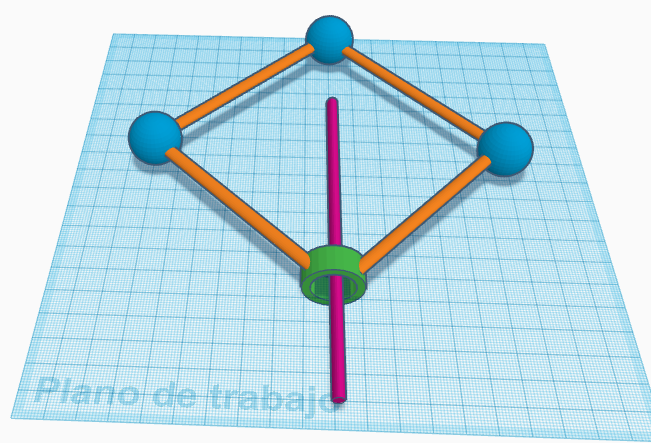
\includegraphics[width=0.35\textwidth]{figures/rotantesAcopladas4.png}
	\end{center}
	


\end{enumerate}
\end{document}
